\documentclass{article}

% UniReps 2026, extended abstract track (non-archival): at most 4 pages of main text.
\usepackage[dblblindworkshop]{neurips_2026}
\workshoptitle{UniReps}
\makeatletter
\renewcommand{\@noticestring}{Submitted to the UniReps Workshop. Do not distribute.}
\makeatother

\usepackage[utf8]{inputenc}
\usepackage[T1]{fontenc}
\usepackage{hyperref}
\usepackage{url}
\usepackage{booktabs}
\usepackage{array}
\usepackage{amsfonts,amsmath,amssymb}
\usepackage{nicefrac}
\usepackage{microtype}
\usepackage{xcolor}
\usepackage{graphicx}
\usepackage{caption}
\graphicspath{{../figures/}}

\newcommand{\dprime}{$d'$}

\title{Transformers Find the Item but Misread It:\\Locating versus Readout in Working Memory}

\author{%
  Anonymous Author(s) \\
  Affiliation \\
  Address \\
  \texttt{email} \\
}

\begin{document}

\maketitle

\begin{abstract}
Large language models (LLMs) show a human-like working-memory limit on the N-back task: performance falls as memory load N grows, and errors concentrate on lures, items that repeat the current letter at a neighboring but incorrect position. Because a transformer keeps the whole sequence in context, the limit must arise when it retrieves an earlier item and uses it. On a \emph{precision} account, softmax attention cannot single out the target, so its neighbors are read instead. On an \emph{interference} account, attention finds the target, but the content of other items corrupts the decision. We test the two accounts in 15 pretrained LLMs from three families (70 million to 14 billion parameters) and find the same answer in every family. The attention heads that carry the task land on the target on most missed matches. Linear probes on the models' activations separate matches from lures almost perfectly (median area under the curve 1.00, against 0.63 for the model's own decision), even on trials where the model falls for the lure. Sharpening attention barely changes sensitivity (\dprime{}), whereas removing the letter identity of non-target items raises it in 42 of 43 model-by-load conditions, more so in larger models. In minimal transformers trained from scratch, a second layer removes the limit. Across families and scales, transformers find the item but misread it.
\end{abstract}

\section{Introduction}
\label{sec:intro}

Working memory, the ability to hold a few pieces of information in mind and use them, is famously limited in humans \citep{cowan2001magical,ma2014changing}. A standard probe is the N-back task \citep{kirchner1958age}: people watch a stream of letters and, for each one, say whether it matches the letter N positions earlier. Performance falls as N grows, and people most often false-alarm on \emph{lures}, letters that repeat the current one at a nearby but wrong distance such as N$\pm$1 \citep{kane2007nback}.

LLMs show the same signature \citep{gong2024chatgpt,hu2025nback,xiong2026superposition}, which is surprising: the whole sequence stays in the model's input, and at every step \emph{attention} \citep{vaswani2017attention} can look back at any earlier item, taking a softmax-weighted average of what earlier positions contain. Because nothing is forgotten, the limit must arise when the model retrieves an item and uses it to decide.

Two accounts have been proposed (Fig.~\ref{fig:overview}b). On the \emph{precision} account \citep{gong2024selfattention}, the model fails to locate the target: softmax makes positions compete for weight \citep{velickovic2025softmax}, the target's neighbors lie only one position away, and weight spills onto them, so the model reads the lure's letter. On the \emph{interference} account \citep{xiong2026superposition}, the model locates the target, but inside the model its content is mixed with that of other recent items, and the mixture corrupts the decision. \citet{xiong2026superposition} found behavioral and representational signatures of interference, but errors biased toward neighbors and trial-averaged attention maps are expected under both accounts. The two predict different things on the trials the model gets wrong: attention off target and gains from sharpening it (precision), or attention on target, the correct information present inside the model, and gains from removing competing content (interference).

We test these predictions in 15 pretrained LLMs. Because every analysis runs in every model, we can also ask whether the mechanism is shared across model families and how it changes with scale. It is shared: the heads that carry the task attend to the target on most errors, a linear probe reads from the model's activations whether a repeated letter sat at the target or at a lure even when the model falls for the lure, and sharpening attention does little while removing distractor content helps, increasingly so with scale. The precision account was proposed for a one-layer transformer, but even there the limit is not positional precision, and a second layer removes it.

\begin{figure}[t]
  \centering
  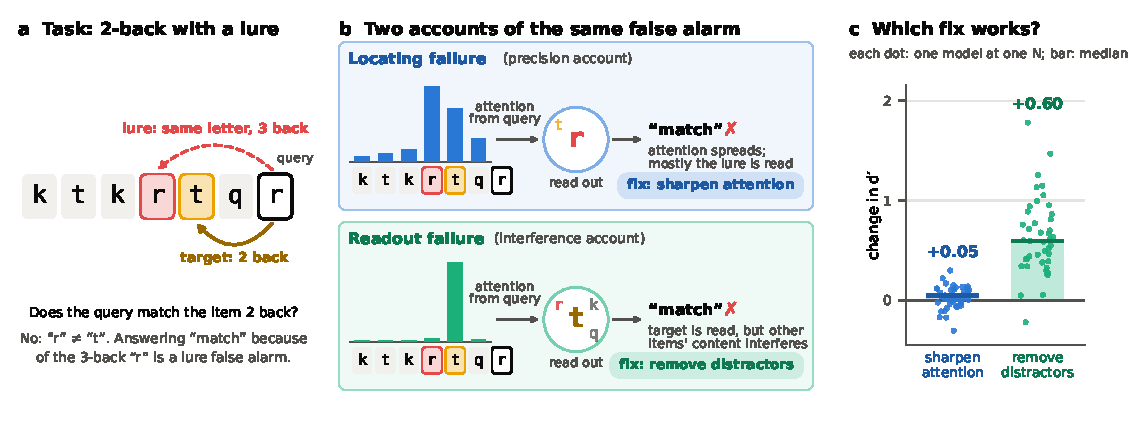
\includegraphics[width=0.94\textwidth]{fig1_overview.pdf}
  \caption{\textbf{Two accounts of the same error.} (a) In 2-back, the query ``r'' must be compared with the item two back (``t''); the ``r'' three back is a lure. (b) Attention lands on the lure and reads its letter (precision account), or lands on the target while other items' letters leak into the decision (interference account). (c) Across 15 LLMs and N = 2--4 (dots: one model at one N; bars: medians), sharpening the attention of the task's most important heads barely changes \dprime{}, whereas removing the letter identity of non-target items raises it in 42 of 43 cases (Section~\ref{sec:causal}).}
  \label{fig:overview}
\end{figure}

\section{Task, models and behavior}
\label{sec:setup}

Each sequence has 24 letters drawn from 20 consonants, including four lures; for each letter (the \emph{query}), the model must say whether it matches the letter N positions back (the \emph{target}). A one-sentence instruction and three solved examples precede the test sequence, one item per line, each holding a letter and its answer (``\texttt{t m}'' for match, ``\texttt{k -}'' for no match); earlier answers are shown correctly, so the model never builds on its own mistakes. The model's decision at each letter is the log-probability difference of ``\texttt{m}'' and ``\texttt{-}'', converted to a yes/no answer by a threshold set on 200 separate calibration sequences; results use 1,000 further sequences per model and N. We report sensitivity \dprime{} from signal detection theory \citep{hautus1995corrections}, which is 0 at chance and is not inflated by a bias toward ``no match''. Models are Pythia 70M--6.9B \citep{biderman2023pythia}, GPT-2 124M--1.5B \citep{radford2019gpt2} and Qwen2.5 0.5B--14B \citep{qwen2025qwen25}. To find the heads that carry the task, we use activation patching \citep{zhang2024patching}: we run two sequences that differ only in the target letter and copy one head's output from one run into the other.

All 15 models decline with N (median \dprime{} 2.57 at N = 1, 0.91 at N = 4, 0.52 at N = 6; Appendix Fig.~\ref{fig:behaviour}, Table~\ref{tab:l2}), and errors concentrate on lures: at N = 2, models answer ``match'' to a median 79\% of N$\pm$1 lures against 4\% of other non-matches. The best-fitting $k$-back rule differs from N in only 14 of 90 cases, all at N$\,\ge\,$4 in small models, so the models are doing N-back rather than drifting to an easier rule.

\section{LLMs find the target but misread it}
\label{sec:locate}

\textbf{Attention lands on the target, even on errors.} We measure how much attention the five most important heads send from the query letter to the target's line and to the lines just before and after it, and say the heads \emph{locate} the target when its line receives at least as much as either neighbor. On correct matches they do so on 88--91\% of trials (median over 14 models), on correct non-matches on about 25\%: the heads search by content, attending to where the query's letter appeared. On misses, matches called ``no match'', the heads look elsewhere on only 16\%, 7\% and 8\% at N = 2, 3 and 4 (Fig.~\ref{fig:locate}a). A classifier trained on correct trials to read the answer from the heads' outputs shows where the answer goes wrong instead: on 41--57\% of misses the outputs already point to the wrong answer although attention was on target, and on 27--43\% they point to the right answer, which is lost in later layers.

\textbf{The model knows where the match was.} On lure false alarms, attention goes to the lure, as a content search should: the query's letter sits there. Avoiding the error requires knowing that the matching letter sat at N$\pm$1 rather than N. We trained linear probes on held-out sequences to tell matches from lures from the residual stream at the query, the running vector that every layer reads from and writes to. The model's own decision separates them barely above chance (median AUC 0.63 at N = 2, 0.58 at N = 3); the probe separates them almost perfectly (1.00 and 0.98 at the best depth; Fig.~\ref{fig:locate}b). A probe on the input embeddings is at chance, so the model computes this information. It is present on the trials the model gets wrong: the probe classifies a median 95\% (N = 2) and 86\% (N = 3) of the model's own lure false alarms as lures (Fig.~\ref{fig:locate}c), and 99.8\% and 95\% in Qwen2.5-14B. The pattern holds in each family (Table~\ref{tab:l7l8}).

\begin{figure}[t]
  \centering
  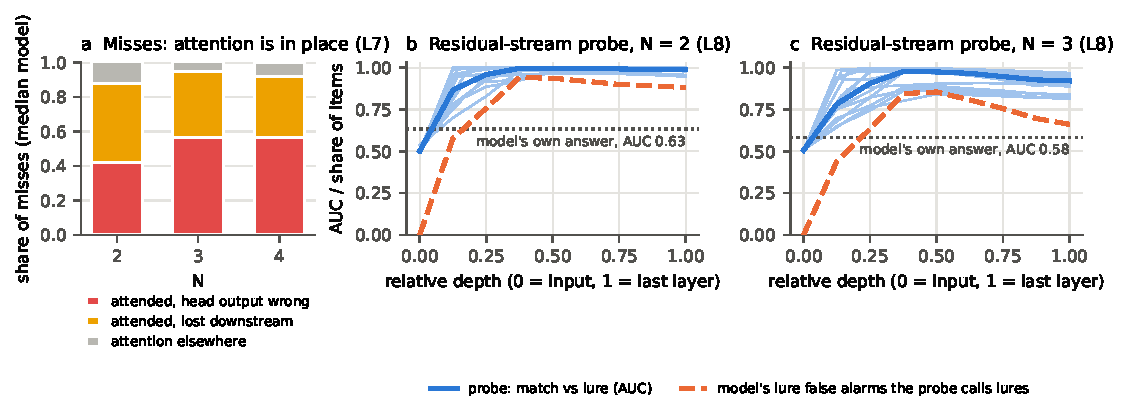
\includegraphics[width=0.94\textwidth]{fig4_locate_vs_readout.pdf}
  \caption{\textbf{LLMs find the target but misread it.} (a) Misses, split by whether the top heads attended to the target and, if so, whether their output already pointed to the wrong answer (median over 14 models). (b, c) A linear probe on the residual stream separates matches from lures (blue; thin lines: models) far better than the model's own decision (dotted), and classifies most of the model's own lure false alarms as lures (orange).}
  \label{fig:locate}
\end{figure}

\section{Removing interference helps; sharpening attention does not}
\label{sec:causal}

We intervene on all 15 models at N = 2--4 on the same sequences, recalibrating the threshold each time and comparing with the unmodified model by a paired bootstrap over sequences (Fig.~\ref{fig:causal}a, Table~\ref{tab:b1}). Two model-by-N conditions where the model is near chance (baseline \dprime{} below 0.3) are excluded, leaving 43. \emph{The identified heads are necessary:} replacing the outputs of the ten most important heads with their mean lowers \dprime{} in 42 of 43 conditions (median $-0.93$); ten random heads from the same layers do nothing ($+0.00$). \emph{Sharper attention barely helps:} dividing the attention scores of the top three heads by $\tau=0.67$ changes \dprime{} by a median $+0.05$ (Wilcoxon $p=0.04$), and when the temperature of every head in the model is changed together, mild \emph{flattening} is best in 19 of 30 conditions. \emph{Removing distractor content helps a lot:} we estimate the 19-dimensional letter-identity subspace from the class means of the 20 letters and, for each query, remove half of every earlier item's component in it, at every layer, sparing only the target. This raises \dprime{} in 42 of 43 conditions (median $+0.60$, up to $+1.78$), lowering false alarms while hits hold. A random subspace of the same size does nothing ($-0.03$), and removing the target's letter instead destroys performance ($-1.54$). Because the intervention uses knowledge of which item is the target, it tests a cause of errors rather than offering a way to fix them. Replicating the letter-direction suppression of \citet{xiong2026superposition} gives a median $+0.11$, about a fifth as much.

Suppression alone does not separate the accounts, because blurring the lure's letter would also remove false alarms caused by attention spilling onto it. What separates them is the combination: attention is on target on errors, the position of the match is linearly decodable on those errors, and sharpening, the remedy the precision account predicts, does little. Forcing the heads' attention onto the target and suppressing only non-lure distractors would test the dissociation more directly and are our next step.

\textbf{Scale weakens the heads, not the interference.} Ablating the identified heads costs less in larger models (Spearman $\rho=0.74$ between size and median change, $p=0.002$): the solution spreads across heads. Removing distractor content helps more ($\rho=0.57$, $p=0.03$; Fig.~\ref{fig:causal}b). In Qwen2.5-14B it raises \dprime{} at N = 3 from 1.60 to 3.38, above the unaided model's 2.42 at N = 2.

\begin{figure}[t]
  \centering
  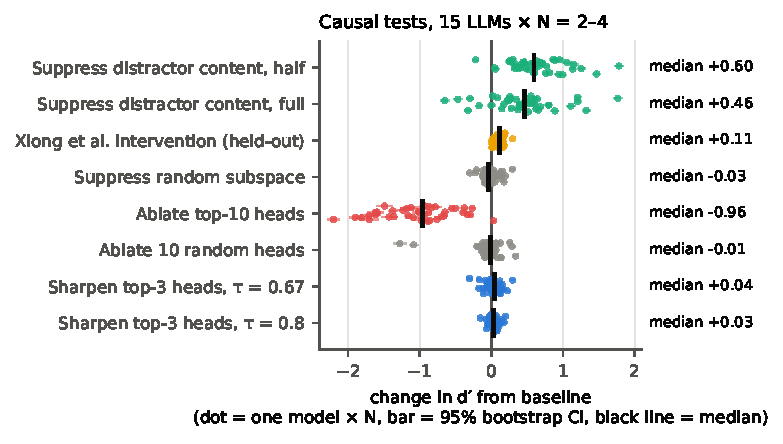
\includegraphics[width=0.94\textwidth]{fig5_causal_tests.pdf}
  \caption{\textbf{Removing interference helps; sharpening attention does not.} (a) Change in \dprime{} under each intervention; dots are one model at one N with 95\% bootstrap intervals, black lines medians. (b) Each model's median change over N = 2--4 against size.}
  \label{fig:causal}
\end{figure}

\section{Where the precision account came from}
\label{sec:minimal}

The precision account was proposed for a single attention layer with no residual stream, trained on N-back \citep{gong2024selfattention}. Such models do decline (\dprime{} 2.67 to 2.15 over N = 1--6; 50 seeds per N; Appendix Fig.~\ref{fig:minimal}). But even here the limit is not positional precision. The output is a weighted average of letter vectors, and no linear readout of such an average with fixed weights can test whether two letters are equal, so a one-layer model must detect a match through \emph{where} its attention goes. Accordingly, replacing its attention by a fixed, perfectly precise split between the query and the target gives \dprime{}~$\approx0$ at every N (720 models, including variants), so precise location without a response to content carries no signal. The position margin, how much higher an attention score an item at distance N receives than one at distance N$\pm$1, predicts neither \dprime{} ($\rho=-0.05$) nor lure false alarms ($\rho=-0.03$) across the 300 main models and does not shrink with N, whereas how much attention to the target changes between match and non-match trials does predict \dprime{} ($\rho=0.62$). Depth removes the constraint: a first layer can copy the letter from N back into the query's position, and a later layer can compare the two directly. With two layers and a residual stream, \dprime{} is 4.5--7.8 at every N with learned, sinusoidal or rotary position codes.

\section{Discussion}
\label{sec:discussion}

Across three model families and two orders of magnitude in size, LLMs locate the item but misread it: the limit lies in readout under interference, not in where attention lands. Like \citet{xiong2026superposition}, we find that transformer working memory resembles interference accounts of human working memory \citep{oberauer2012interference,szmalec2011interference}, in which items are available but compete at the moment of use. The gap between what a probe reads from the model's activations and what the model's decision uses is also a caution for comparing representations across systems: information that is decodable from a population need not be the information that drives behavior.

\textbf{Limitations.} We study one task, letter N-back with synthetic stimuli, in models up to 14B parameters. The locating criterion compares the target only with its two neighbors. Distractor suppression uses knowledge of which item is the target, so it diagnoses the cause of errors rather than offering a way to fix them. The probes show that information is linearly present, not that the model could use it with its existing weights.

\bibliographystyle{plainnat}
\bibliography{refs}

\appendix

\section{Methods}
\label{app:methods}

\textbf{LLM evaluation.} Prompts start with a one-sentence instruction and ``N = $n$'', then three demonstration sequences with correct answers and the test sequence. Letters, ``\texttt{ m}'' and ``\texttt{ -}'' are single tokens in every tokenizer (checked per model). Models up to 1B run in float32 and larger models in bfloat16. The chat format, used for Qwen2.5-Instruct 0.5B--7B, sends one user turn per letter and one assistant turn per answer.

\textbf{Head ranking.} Clean and corrupted prompts differ only in the letter at $i-N$, flipping the answer. For each head we patch its output from the clean into the corrupted run at all positions and report the recovered fraction of the mean logit-difference gap. At N = 2 the top head alone recovers 16--73\% of the gap, depending on the model.

\textbf{Locating analysis.} Attention from the query letter token to all tokens of a line is summed per head and averaged over the top five heads. GPT-2 Large is excluded because its top heads attend to none of the three lines. The answer classifier is a logistic regression on the top five heads' outputs at the query, trained on up to 4,000 correct items and applied to errors.

\textbf{Probe.} Items with a same-letter item at $i-N$ (matches) or at a lure distance (lures); logistic regression with $L_2$ penalty on standardized features at nine depths, five folds split by sequence. Probe and model are scored by the area under the ROC curve (AUC).

\textbf{Interventions.} Sharpening multiplies a head's attention scores by $1/\tau$; ablation replaces a head's output by its mean over calibration items; random heads are drawn from the same layers. Suppression replaces $h$ by $h-\alpha\,((h-\mu)U)U^\top$ with $\alpha=0.5$ at every residual site (the input to the first layer and every layer's output) over the tokens of each non-target line, where $U$ spans the 19 centered class means of the 20 letters at test-item letter tokens, estimated on calibration sequences. Full suppression ($\alpha=1$) also helps (median $+0.46$) but over-suppresses in Qwen2.5-7B. The random control uses a random orthonormal $U$ of the same rank. Each intervention is compared with the unmodified model by a paired bootstrap over sequences (2,000 resamples). For the replication of \citet{xiong2026superposition}, one letter direction is removed at one of the two earliest depths at answer positions only, with the configuration chosen on held-out calibration sequences.

\textbf{Minimal models.} Attention-only transformers ($d_{\text{model}}=512$ for the main one-layer configuration, 128 for variants), Adam with learning rate $10^{-4}$, batch 32, fresh sequences each step, up to 30,000 steps with early stopping. 50 seeds for the main configuration and 10 per variant (width, training-set size, weight decay, depth, position code). The 720 one-layer models used for attention edits are the main configuration and seven variants at N = 1--6; the score decomposition and correlations use the main configuration alone (300 models).

\section{Additional figures and tables}
\label{app:results}

\begin{figure}[h]
  \centering
  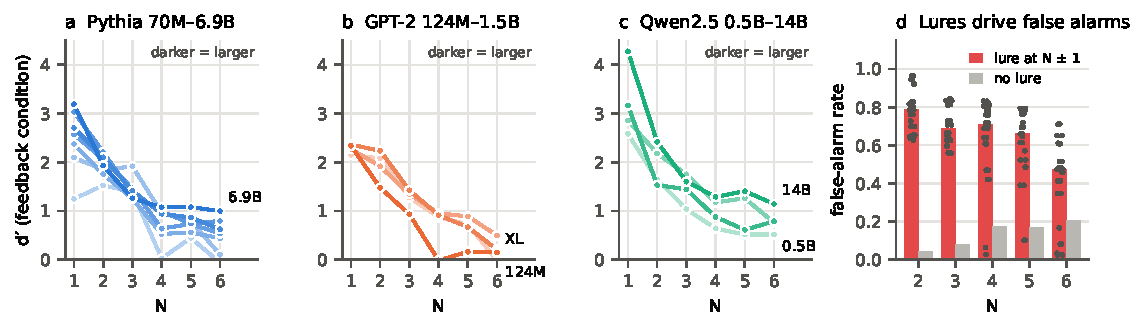
\includegraphics[width=\textwidth]{fig3_llm_behaviour.pdf}
  \caption{\textbf{LLMs decline with N and fall for lures.} (a--c) \dprime{} against N for three families; darker lines are larger models. (d) False-alarm rates on N$\pm$1 lures (red; dots are models) and on other non-matches (gray), medians over 15 models.}
  \label{fig:behaviour}
\end{figure}

\begin{figure}[h]
  \centering
  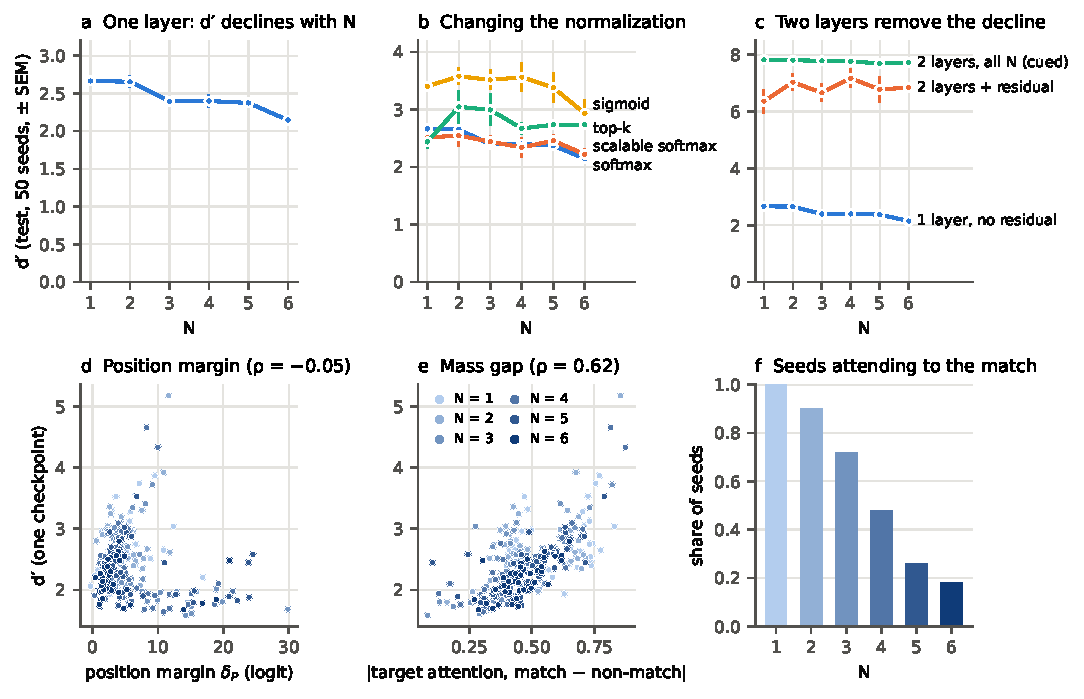
\includegraphics[width=\textwidth]{fig2_minimal_models.pdf}
  \caption{\textbf{Minimal transformers trained from scratch.} (a) A one-layer model without residual stream declines with N (50 seeds, $\pm$SEM). (b) Sigmoid and top-$k$ attention flatten the decline; scalable softmax \citep{nakanishi2025scalable} does not. (c) Two layers with a residual stream remove it, for one model per N and for one cued model trained on all N. (d, e) Across 300 one-layer models (darker = larger N), \dprime{} is unrelated to the position margin but tracks how much attention to the target differs between match and non-match trials. (f) Share of models that attend more to the target on match trials.}
  \label{fig:minimal}
\end{figure}

\begin{table}[h]
  \centering\small
  \caption{\dprime{} by model and N, and false-alarm rates on N$\pm$1 lures versus other non-matches at N = 2.}
  \label{tab:l2}
  \begin{tabular}{lrrrrrrr}
\toprule
Model & $N{=}1$ & 2 & 3 & 4 & 5 & 6 & lure FA, $N{=}2$ \\
\midrule
Pythia-70m & 1.25 & 1.52 & 1.40 & 0.03 & 0.45 & -0.06 & 0.83 / 0.12 \\
Pythia-160m & 2.10 & 1.85 & 1.92 & 0.96 & 0.79 & 0.10 & 0.79 / 0.02 \\
Pythia-410m & 2.37 & 1.76 & 1.25 & 0.53 & 0.56 & 0.44 & 0.76 / 0.04 \\
Pythia-1b & 2.57 & 2.06 & 1.46 & 0.64 & 0.73 & 0.54 & 0.83 / 0.04 \\
Pythia-1.4b & 3.03 & 2.21 & 1.36 & 0.99 & 0.74 & 0.80 & 0.73 / 0.02 \\
Pythia-2.8b & 2.71 & 2.10 & 1.42 & 0.94 & 0.87 & 0.63 & 0.82 / 0.03 \\
Pythia-6.9b & 3.19 & 1.93 & 1.26 & 1.07 & 1.08 & 1.00 & 0.64 / 0.03 \\
GPT-2 & 2.15 & 2.08 & 1.28 & 0.87 & 0.73 & -0.02 & 0.96 / 0.08 \\
GPT-2 medium & 2.27 & 1.92 & 1.35 & 0.95 & 0.89 & 0.50 & 0.92 / 0.06 \\
GPT-2 large & 2.36 & 2.24 & 1.43 & 0.91 & 0.67 & 0.21 & 0.95 / 0.04 \\
GPT-2 xl & 2.34 & 1.48 & 0.93 & -0.01 & 0.16 & 0.15 & 0.70 / 0.06 \\
Qwen2.5-0.5B & 2.58 & 1.64 & 1.04 & 0.64 & 0.52 & 0.52 & 0.81 / 0.06 \\
Qwen2.5-1.5B & 2.86 & 2.18 & 1.75 & 1.18 & 1.26 & 0.76 & 0.65 / 0.01 \\
Qwen2.5-7B & 3.17 & 1.53 & 1.44 & 0.88 & 0.61 & 0.79 & 0.64 / 0.06 \\
Qwen2.5-14B & 4.28 & 2.42 & 1.60 & 1.29 & 1.41 & 1.15 & 0.63 / 0.01 \\
\bottomrule
\end{tabular}

\end{table}

\begin{table}[h]
  \centering\small
  \caption{Change in \dprime{} under each intervention; bold entries have 95\% bootstrap intervals excluding zero. $^\dagger$ degenerate baseline (excluded from summaries).}
  \label{tab:b1}
  \begin{tabular}{lrrrrrrr}
\toprule
Model & $N$ & base $d'$ & sharpen & ablate top & ablate rand. & suppress & supp. rand. \\
\midrule
Pythia-70m & 2 & 1.52 & \textbf{-0.11} & \textbf{-1.71} & \textbf{-1.08} & \textbf{+0.38} & \textbf{-0.30} \\
 & 3 & 1.40 & \textbf{+0.22} & \textbf{-1.49} & \textbf{-1.28} & \textbf{+0.05} & \textbf{-0.21} \\
 & 4 & 0.03$^\dagger$ & \textbf{+0.97} & \textbf{-0.17} & +0.04 & \textbf{+0.82} & \textbf{+0.31} \\
\addlinespace[2pt]
Pythia-160m & 2 & 1.85 & \textbf{+0.14} & \textbf{-1.62} & +0.01 & \textbf{+1.25} & \textbf{+0.29} \\
 & 3 & 1.92 & \textbf{-0.17} & \textbf{-1.90} & \textbf{-0.13} & \textbf{+0.30} & +0.03 \\
 & 4 & 0.96 & \textbf{+0.30} & \textbf{-1.09} & \textbf{-0.20} & \textbf{-0.22} & +0.01 \\
\addlinespace[2pt]
Pythia-410m & 2 & 1.76 & \textbf{+0.17} & \textbf{-1.36} & \textbf{-0.03} & \textbf{+0.61} & -0.01 \\
 & 3 & 1.25 & \textbf{-0.08} & \textbf{-1.18} & \textbf{+0.13} & \textbf{+0.60} & \textbf{-0.04} \\
 & 4 & 0.53 & \textbf{+0.13} & \textbf{-0.39} & \textbf{+0.08} & \textbf{+0.70} & \textbf{+0.05} \\
\addlinespace[2pt]
Pythia-1b & 2 & 2.06 & \textbf{-0.04} & \textbf{-1.81} & \textbf{+0.13} & \textbf{+0.59} & \textbf{-0.05} \\
 & 3 & 1.46 & \textbf{+0.11} & \textbf{-1.70} & \textbf{+0.34} & \textbf{+0.26} & \textbf{-0.12} \\
 & 4 & 0.64 & \textbf{+0.09} & \textbf{-0.83} & \textbf{+0.29} & \textbf{+0.39} & \textbf{-0.09} \\
\addlinespace[2pt]
Pythia-1.4b & 2 & 2.21 & \textbf{+0.08} & \textbf{-1.61} & \textbf{-0.06} & \textbf{+0.95} & \textbf{-0.05} \\
 & 3 & 1.36 & \textbf{+0.05} & \textbf{-0.93} & \textbf{+0.05} & \textbf{+0.46} & \textbf{+0.05} \\
 & 4 & 0.99 & \textbf{+0.05} & \textbf{-0.66} & +0.02 & \textbf{+0.44} & \textbf{-0.07} \\
\addlinespace[2pt]
Pythia-2.8b & 2 & 2.10 & \textbf{-0.05} & \textbf{-1.59} & \textbf{-0.12} & \textbf{+0.25} & \textbf{-0.03} \\
 & 3 & 1.42 & \textbf{+0.12} & \textbf{-1.01} & \textbf{-0.03} & \textbf{+0.34} & -0.01 \\
 & 4 & 0.94 & \textbf{+0.12} & \textbf{-0.70} & \textbf{+0.02} & \textbf{+0.41} & \textbf{+0.05} \\
\addlinespace[2pt]
Pythia-6.9b & 2 & 1.93 & \textbf{+0.03} & \textbf{-1.02} & \textbf{-0.08} & \textbf{+0.94} & \textbf{-0.08} \\
 & 3 & 1.26 & \textbf{+0.10} & \textbf{-0.34} & \textbf{+0.26} & \textbf{+1.47} & \textbf{+0.13} \\
 & 4 & 1.07 & \textbf{+0.07} & \textbf{-0.55} & +0.03 & \textbf{+1.13} & \textbf{+0.09} \\
\addlinespace[2pt]
GPT-2 & 2 & 2.08 & \textbf{-0.30} & \textbf{-2.20} & \textbf{-0.09} & \textbf{+0.05} & \textbf{-0.22} \\
 & 3 & 1.28 & -0.00 & \textbf{-1.12} & \textbf{-0.09} & \textbf{+0.71} & \textbf{-0.07} \\
 & 4 & 0.87 & \textbf{-0.02} & \textbf{-0.86} & \textbf{+0.07} & \textbf{+0.32} & \textbf{-0.12} \\
\addlinespace[2pt]
GPT-2 medium & 2 & 1.92 & +0.02 & \textbf{-1.38} & \textbf{+0.14} & \textbf{+1.05} & +0.00 \\
 & 3 & 1.35 & \textbf{-0.06} & \textbf{-1.43} & \textbf{-0.10} & \textbf{+0.86} & \textbf{-0.08} \\
 & 4 & 0.95 & \textbf{-0.07} & \textbf{-0.98} & \textbf{-0.18} & \textbf{+0.34} & \textbf{-0.12} \\
\addlinespace[2pt]
GPT-2 large & 2 & 2.24 & \textbf{-0.17} & \textbf{-1.16} & \textbf{-0.09} & \textbf{+0.68} & \textbf{+0.06} \\
 & 3 & 1.43 & \textbf{+0.15} & \textbf{-0.89} & \textbf{+0.02} & \textbf{+0.77} & \textbf{-0.03} \\
 & 4 & 0.91 & \textbf{+0.06} & \textbf{-0.50} & \textbf{-0.05} & \textbf{+0.55} & \textbf{-0.03} \\
\addlinespace[2pt]
GPT-2 xl & 2 & 1.46 & \textbf{+0.12} & \textbf{-1.24} & \textbf{-0.06} & \textbf{+0.52} & \textbf{+0.15} \\
 & 3 & 0.94 & \textbf{+0.12} & \textbf{-0.88} & +0.01 & \textbf{+0.81} & \textbf{-0.05} \\
 & 4 & -0.02$^\dagger$ & \textbf{+0.55} & \textbf{-0.16} & \textbf{+0.53} & \textbf{+0.91} & \textbf{+0.48} \\
\addlinespace[2pt]
Qwen2.5-0.5B & 2 & 1.64 & \textbf{-0.03} & \textbf{-0.87} & \textbf{+0.06} & \textbf{+0.49} & \textbf{+0.15} \\
 & 3 & 1.04 & \textbf{+0.05} & \textbf{-0.65} & \textbf{-0.11} & \textbf{+0.67} & \textbf{-0.07} \\
 & 4 & 0.64 & -0.01 & \textbf{-0.38} & +0.02 & \textbf{+0.60} & \textbf{-0.09} \\
\addlinespace[2pt]
Qwen2.5-1.5B & 2 & 2.18 & \textbf{+0.10} & \textbf{-0.76} & \textbf{+0.06} & \textbf{+0.89} & \textbf{-0.11} \\
 & 3 & 1.75 & +0.01 & \textbf{-0.93} & \textbf{-0.05} & \textbf{+1.15} & +0.01 \\
 & 4 & 1.18 & \textbf{-0.04} & \textbf{-0.78} & \textbf{-0.11} & \textbf{+0.28} & \textbf{-0.09} \\
\addlinespace[2pt]
Qwen2.5-7B & 2 & 1.53 & +0.01 & \textbf{-0.27} & \textbf{+0.06} & \textbf{+0.41} & \textbf{+0.04} \\
 & 3 & 1.44 & \textbf{-0.11} & \textbf{-0.29} & -0.02 & \textbf{+0.99} & \textbf{+0.20} \\
 & 4 & 0.88 & +0.00 & +0.03 & +0.00 & \textbf{+0.63} & \textbf{+0.14} \\
\addlinespace[2pt]
Qwen2.5-14B & 2 & 2.42 & \textbf{+0.05} & \textbf{-0.48} & \textbf{-0.04} & \textbf{+0.46} & \textbf{-0.10} \\
 & 3 & 1.60 & +0.01 & \textbf{-0.17} & +0.01 & \textbf{+1.78} & \textbf{-0.05} \\
 & 4 & 1.29 & \textbf{+0.13} & \textbf{-0.21} & \textbf{+0.07} & \textbf{+0.76} & \textbf{+0.18} \\
\addlinespace[2pt]
\bottomrule
\end{tabular}

\end{table}

\begin{table}[h]
  \centering\small
  \caption{Locating analysis (share of misses with attention off target, on target but lost in later layers, or on target with the heads' output already wrong) and probe results (AUC of the model's own decision and of the probe for matches versus lures, and share of the model's lure false alarms the probe classifies as lures) per model.}
  \label{tab:l7l8}
  \setlength{\tabcolsep}{4.5pt}
  \begin{tabular}{lrrrrrrr}
\toprule
& & \multicolumn{3}{c}{L7: share of misses} & \multicolumn{3}{c}{L8: match vs.\ lure} \\
\cmidrule(lr){3-5}\cmidrule(lr){6-8}
Model & $N$ & elsewhere & lost later & head wrong & model AUC & probe AUC & FA called lure \\
\midrule
Pythia-70m & 2 & 0.08 & 0.49 & 0.43 & 0.58 & 0.97 & 0.75 \\
 & 3 & 0.01 & 0.42 & 0.57 & 0.57 & 0.91 & 0.61 \\
Pythia-160m & 2 & 0.26 & 0.34 & 0.40 & 0.63 & 0.98 & 0.82 \\
 & 3 & 0.03 & 0.59 & 0.38 & 0.58 & 0.99 & 0.85 \\
Pythia-410m & 2 & 0.11 & 0.36 & 0.53 & 0.66 & 1.00 & 0.95 \\
 & 3 & 0.06 & 0.40 & 0.54 & 0.58 & 0.98 & 0.84 \\
Pythia-1b & 2 & 0.11 & 0.32 & 0.57 & 0.68 & 1.00 & 0.95 \\
 & 3 & 0.06 & 0.30 & 0.64 & 0.60 & 0.98 & 0.87 \\
Pythia-1.4b & 2 & 0.12 & 0.72 & 0.16 & 0.76 & 1.00 & 0.99 \\
 & 3 & 0.06 & 0.38 & 0.56 & 0.62 & 0.99 & 0.92 \\
Pythia-2.8b & 2 & 0.04 & 0.36 & 0.60 & 0.71 & 1.00 & 1.00 \\
 & 3 & 0.04 & 0.38 & 0.58 & 0.60 & 1.00 & 0.96 \\
Pythia-6.9b & 2 & 0.19 & 0.55 & 0.26 & 0.74 & 1.00 & 1.00 \\
 & 3 & 0.08 & 0.38 & 0.54 & 0.60 & 1.00 & 0.98 \\
GPT-2 & 2 & 0.16 & 0.65 & 0.19 & 0.49 & 0.97 & 0.84 \\
 & 3 & 0.12 & 0.38 & 0.50 & 0.48 & 0.84 & 0.53 \\
GPT-2 medium & 2 & 0.18 & 0.53 & 0.29 & 0.48 & 0.99 & 0.87 \\
 & 3 & 0.07 & 0.39 & 0.54 & 0.47 & 0.86 & 0.57 \\
GPT-2 large & 2 & 0.72 & 0.15 & 0.13 & 0.56 & 0.99 & 0.92 \\
 & 3 & 0.54 & 0.20 & 0.26 & 0.50 & 0.88 & 0.59 \\
GPT-2 xl & 2 & 0.15 & 0.42 & 0.43 & 0.60 & 1.00 & 0.92 \\
 & 3 & 0.10 & 0.28 & 0.62 & 0.49 & 0.89 & 0.69 \\
Qwen2.5-0.5B & 2 & 0.16 & 0.50 & 0.34 & 0.62 & 1.00 & 1.00 \\
 & 3 & 0.09 & 0.23 & 0.67 & 0.53 & 0.99 & 0.91 \\
Qwen2.5-1.5B & 2 & 0.17 & 0.42 & 0.41 & 0.78 & 1.00 & 1.00 \\
 & 3 & 0.04 & 0.39 & 0.57 & 0.67 & 0.99 & 0.86 \\
Qwen2.5-7B & 2 & 0.14 & 0.43 & 0.43 & 0.63 & 1.00 & 0.98 \\
 & 3 & 0.45 & 0.19 & 0.36 & 0.60 & 0.98 & 0.88 \\
Qwen2.5-14B & 2 & 0.68 & 0.17 & 0.14 & 0.81 & 1.00 & 1.00 \\
 & 3 & 0.51 & 0.13 & 0.36 & 0.64 & 1.00 & 0.95 \\
\bottomrule
\end{tabular}

\end{table}

\end{document}
